\section{Introduction partielle}
$ _{} $ $ _{} $ $ _{} $ $ _{} $ $ _{} $Le résumé automatique étant le sujet principal de ce mémoire, dans cette partie nous le présentons alors en détail en tant que discipline et tâche du \textit{NLP}. Nous allons ici présenter les théories sur la synthèse automatique des textes, en classifiant les diverses méthodes utilisées, afin de pouvoir situer notre système dans l'ensemble des travaux jusque-là menés sur ce sujet.

Ensuite, nous présenterons les diverses approches utilisées pour le résumé automatique, sans oublier d'approfondir notre présentation des modèles de type \textit{transformer} adaptés à cette tâche, pour finalement mentionner le modèle que nous estimons le plus adapté concernant l'approche basée sur le \textit{deep-learning} pour la synthèse automatique.\\
Enfin, nous allons réaliser une conception rapide mais suffisante de l'architecture globale de notre système, que nous appellerons \textbf{\textit{Mon Résumeur}}, tout en précisant le rôle et le fonctionnement de chaque partie.
\section{Présentation et définitions}
$ _{} $ $ _{} $ $ _{} $ $ _{} $ $ _{} $Selon Le Petit Robert, résumer c'est reprendre en plus court un discours, le présenter brièvement en conservant l'essentiel. En d'autres termes, c'est l'abréger, l'écourter, le réduire.
De même, en tant qu'exercice intellectuel, le résumé, consiste à réduire un texte tout en lui restant fidèle. Il exige donc de restituer les idées en un nombre déterminé de mots,  en évitant au mieux de recopier le texte à résumer. Il faut alors composer un texte plus court qui contienne l'essentiel du message initial \cite{fasoEduc}.\\
De cela on tire que le résumé devient automatique s'il est généré par un logiciel ou un système informatique.\\
$ _{} $ $ _{} $ $ _{} $ $ _{} $ $ _{} $Cette définition est en fait correcte bien qu'elle ne soit pas assez précise pour notre contexte. Il nous faut une définition assez générale et précise, embrassant au mieux l'aspect automatique, ou mieux, l'aspect informatique, qui nous intéresse dans ce mémoire.\\
Une définition assez valable est celle de Torres-Moreno Juan-Manuel qui dit qu'\textit{un résumé automatique est un texte généré par un logiciel, cohérent et contenant une partie im\-por\-tan\-te des informations pertinentes de la source, et dont le taux de compression est inférieur au tiers de la taille du(des) document(s) source(s)} \cite{torres2014automatic}.\\
$ _{} $ $ _{} $ $ _{} $ $ _{} $ $ _{} $L'introduction du taux de compression dans la définition n'est pas anodine car, on s'est très vite rendu compte que la performance d'un système de résumé automatique dépendait fortement du taux de compression. En effet, les études de \cite{Lin1999TrainingAS} montrent que les meilleures performances des systèmes de résumé automatique sont généralement atteintes pour des taux de compression compris entre $ 15 $ et $ 30\% $ \cite{torres2014automatic}.\\
$ _{} $ $ _{} $ $ _{} $ $ _{} $ $ _{} $Nous allons adopter, dans ce travail, la définition de Torres-Moreno Juan-Manuel ci-haut présentée.\\

Toutefois, on ne doit pas manquer de signaler que la génération automatique des résumés est un problème complexe en soi, tout comme l'évaluation des résultats. Le résumé est en effet une tâche cognitive requérant la compréhension du texte considéré et, les humains n'étant pas toujours bons dans les tâches de synthèse, le manque d'étalon explique qu'il y ait également une difficulté d'automatisation du processus.
\section{Catégorisation des résumés}
$ _{} $ $ _{} $ $ _{} $ $ _{} $ $ _{} $Les résumés peuvent être classifiés selon différents critères tels que leur fonction, le nombre de documents source, le genre de document, le type de résumé, le type de résumeur, le contexte,...\\
Parcourons de manière succincte ces différents critères de classification \cite{MaaliMnasri,maaloul:tel-00756111,mani2001automatic,Nenkova,moens2001automatic,torres2014automatic}
:
\subsection{Selon la fonction}
$ _{} $ $ _{} $ $ _{} $ $ _{} $ $ _{} $Selon leur fonction, on classifie les résumés en deux groupes qui sont le \textit{résumé indicatif} et le \textit{résumé informatif}.
\subsubsection{Résumé indicatif}
$ _{} $ $ _{} $ $ _{} $ $ _{} $ $ _{} $Tel une table des matières, un résumé indicatif renseigne le lecteur sur les thèmes abordés dans un document. Il liste donc les sujets les plus importants évoqués par le texte. Certains systèmes de résumé guidé génèrent un résumé indicatif du texte comme étape initiale, l'utilisateur choisit alors parmi les sujets proposés par le résumé ceux qui l'intéressent et le système produit enfin un résumé informatif du texte, guidé par la requête de l'utilisateur. La requête dans ce cas est l'ensemble des sujets sélectionnés à partir du résumé indicatif.
\subsubsection{Résumé informatif}
$ _{} $ $ _{} $ $ _{} $ $ _{} $ $ _{} $Il s'agit d'un modèle rétréci du texte d'origine, relatant le plus largement possible les informations contenues dans celui-ci. Ce type de résumé répond souvent à une attente en résumant de plus le contenu. La problématique ici est donc double : comprendre ce qui n'est pas information dans un texte et connaître le besoin de l'utilisateur final.\\
Néanmoins, si on n'a pas de requête spécifique de la part de l'utilisateur, le résumé informatif est réalisé en veillant à ce que l'ensemble des principaux sujets du texte d'origine soit rapporté. Ainsi, les sujets principaux qui sont rappelés dans le résumé sont répartis de manière fidèle par rapport à l'organisation initiale afin de donner un juste aperçu du texte source.\newpage
\subsection{Selon le nombre de documents sources}
$ _{} $ $ _{} $ $ _{} $ $ _{} $ $ _{} $Selon le nombre de documents sources on a les résumés mono-document et multi-document.
\subsubsection{Résumé mono-document}
$ _{} $ $ _{} $ $ _{} $ $ _{} $ $ _{} $Il consiste à résumer un document isolé. Le corpus de documents source est donc ici constitué d'un seul et unique document. 
\subsubsection{Résumé multi-documents}
$ _{} $ $ _{} $ $ _{} $ $ _{} $ $ _{} $Il s'agit d'un résumé de plusieurs documents (un groupe de documents), très souvent liés thé\-ma\-ti\-que\-ment, en faisant attention à ne pas insérer des informations déjà évoquées.
\subsection{Selon le genre des documents}
\subsubsection{Résumé des documents journalistiques}
$ _{} $ $ _{} $ $ _{} $ $ _{} $ $ _{} $Il s'agit de résumer les documents du type article de presse (sachant qu'ils ont une structure particulière). En effet, on sait par exemple que dans le domaine journalistique, les informations les plus importantes sont souvent mentionnées au début du texte.\cite{MaaliMnasri}
\subsubsection{Résumé des documents spécialisés}
$ _{} $ $ _{} $ $ _{} $ $ _{} $ $ _{} $Il s'agit de résumer des documents en provenance d'un domaine précis (géologie, médecine, mathématique,...), fortement spécialisé.
\subsubsection{Résumé des documents littéraires}
$ _{} $ $ _{} $ $ _{} $ $ _{} $ $ _{} $C'est le résumé de documents du type narratif, des textes littéraires, des textes ar\-gu\-men\-ta\-tifs, ...
\subsubsection{Résumé des documents encyclopédiques}
$ _{} $ $ _{} $ $ _{} $ $ _{} $ $ _{} $Ici il s'agit de résumer des documents de type encyclopédique (en général multi-thématiques de toute évidence) à l'exemple de Wikipédia...
\subsection{Selon le type de sortie (résumé obtenu)}
$ _{} $ $ _{} $ $ _{} $ $ _{} $ $ _{} $Cette classification est très importante et très utilisée. Il s'agit des :
\subsubsection{Résumé extractif (\textit{extractive summarization})}
$ _{} $ $ _{} $ $ _{} $ $ _{} $ $ _{} $Le résumé extrait est formé de segments de texte extraits du(des) document(s) source(s). Ces segments peuvent être des phrases, des propositions ou n'importe quelle unité textuelle présent dans le(s) document(s) à résumer. Le problème consiste donc à repérer les segments de texte qui semblent être les plus pertinents pour faire partie du résumé final. Les éléments obtenus à la fin sont donc explicitement présents dans le(s) document(s) source(s).
\subsubsection{Résumé abstractif (\textit{abstractive summarization})}
$ _{} $ $ _{} $ $ _{} $ $ _{} $ $ _{} $Les méthodes de résumé abstractives imitent, jusqu'à un certain degré, le processus naturel accompli par l'homme pour résumer un document. Par conséquent, elles produisent des résumés plus similaires aux résumés manuels (humains). Ce processus peut être décrit par deux étapes majeures : la compréhension du texte source et la génération du résumé. La première étape vise à analyser sé\-man\-ti\-que\-ment le contenu du texte et à identifier les parties à exprimer dans le résumé. C'est en quelques sortes une tâche d'extraction d'information liée au domaine abordé ou de regroupement des phrases du texte source. Vient ensuite la génération du texte.\\
Bref, on produit un résumé rapportant le contenu du(des) texte(s) source(s) en utilisant un vocabulaire souvent différent et plus concis.\\

Il existe aussi des résumés dits \textit{semi-extractifs}, et même aussi des résumés dits \textit{par compression} \cite{torres2014automatic} mais nous estimons inutile de les décrire ici étant donné que la distinction abstractif-extractif suffit pour notre contexte.
\subsection{Selon le type de résumeur}
$ _{} $ $ _{} $ $ _{} $ $ _{} $ $ _{} $Le résumeur est le système qui réalise le résumé. Il peut s'agir d'une entité naturelle (un humain) ou artificielle (un logiciel). On a donc es\-sen\-tiel\-lement les deux cas suivants :
\subsubsection{Résumé humain (manuel)}
$ _{} $ $ _{} $ $ _{} $ $ _{} $ $ _{} $Il s'agit d'un résumé réalisé par un humain. Il peut être fait par l'auteur même du document (on parle souvent de \textit{résumé d'auteur}), par un expert du domaine traité (on parle souvent de \textit{résumé d'expert}) ou par un professionnel de résumé (on parle de \textit{résumé professionnel}).
\subsubsection{Résumé automatique}
$ _{} $ $ _{} $ $ _{} $ $ _{} $ $ _{} $Il s'agit, comme on l'a maintes fois mentionné, d'un résumé fait par un système informatique.
\subsection{Selon le contexte}
\subsubsection{Résumé générique}
$ _{} $ $ _{} $ $ _{} $ $ _{} $ $ _{} $Ici on résume le document sans prendre en compte les besoins d'information de l'utilisateur. On produit juste un résumé complet et le plus mieux fait possible.
\subsubsection{Résumé guidé}
$ _{} $ $ _{} $ $ _{} $ $ _{} $ $ _{} $Pour ces types de résumé, l'utilisateur commande la génération du résumé en précisant les types d'information dont il a besoin.
\subsubsection{Résumé mis à jour}
$ _{} $ $ _{} $ $ _{} $ $ _{} $ $ _{} $Il s'agit d'un résumé de type dynamique par essence. Ici, un ensemble de documents sources est résumé en veillant minutieusement à ce que le document dont le résumé est ajouté à la suite d'un précédent résumé ne puisse pas créer une répétition d'information. Il y a donc un contrôle de nouveauté.\newpage
\subsection{Selon le destinataire du résumé}
$ _{} $ $ _{} $ $ _{} $ $ _{} $ $ _{} $On peut aussi classifier un résumé selon le public auquel il est destiné.
\subsubsection{Résumé sans profil}
$ _{} $ $ _{} $ $ _{} $ $ _{} $ $ _{} $Il s'agit d'un résumé qui ne tient pas compte d'un quelconque profil utilisateur. Le résumé est donc généré sans tenir compte de la personnalité des utilisateurs.
\subsubsection{Résumé avec profil}
$ _{} $ $ _{} $ $ _{} $ $ _{} $ $ _{} $Il s'agit d'un résumé dont l'un des éléments guides (requête) est le profil des individus auxquels le résumé est destiné.\\

\textbf{En ce qui concerne notre système, nous implémenterons à la fois un résumeur abstractif et un résumeur extractif et ce sera mono-document. En plus de cela, le résumé ne sera pas guidé, il s'agira de produire des résumés génériques, pour des documents de type littéraire (documents du type narratif, des textes littéraires, des textes argumentatifs,...).}
\section{Approches de résumé automatique}
$ _{} $ $ _{} $ $ _{} $ $ _{} $ $ _{} $Nous allons présenter ici diverses approches algorithmiques pour résumer les documents textuels. Les approches seront abordées en supposant que les résumés sont prin\-ci\-pa\-le\-ment classés en \textit{abstractif} et \textit{extractif}.
\subsection{Techniques intuitives de résumé \cite{MaaliMnasri}}
$ _{} $ $ _{} $ $ _{} $ $ _{} $ $ _{} $Avec des \textbf{critères centrés sur le contenu des textes}, il existe un grand nombre d'al\-go\-ri\-thmes assez triviaux de résumé, qui sont basés entre autres sur :
\begin{itemize}
\item[•] La fréquence d'occurrence des mots et
\item[•] L'annotation en rôle sémantique.
\end{itemize}
Ces critères mettent l'accent sur le contenu du texte et le message qu'il communique.
\subsubsection{Fréquence d'occurrence des mots}
$ _{} $ $ _{} $ $ _{} $ $ _{} $ $ _{} $L'idée majeure des techniques qui utilisent ce critère consiste à considérer que les mots les plus fréquents sont les plus liés au sujet principal du texte à résumer. Cette approche assez simpliste mais fonctionnelle fut introduite en $ 1958 $ par \textbf{Luhn} \cite{Luhn58}, une première tentative de résumé automatique.\\
On affecte des scores aux phrases présentes dans le texte, en additionnant chaque fois les poids des mots les constituant (on attribue ce poids en fonction de la fréquence d'apparition du mot considéré dans le texte entier). Et, à la fin, le résumé est constitué avec les phrases extraites du texte source, et dont le score dépasse un certain seuil dépendant de la taille maximale imposée pour le résumé. Le tout est finalement réarrangé selon l'ordre d'apparition (des phrases sélectionnées) dans le texte d'origine.
\subsubsection{L'annotation en rôle sémantique}
$ _{} $ $ _{} $ $ _{} $ $ _{} $ $ _{} $Ici, l'idée est simple. En utilisant des techniques de repérage d'entités nommées (voir le chapitre précédent), on identifie les entités présentes dans le document. Après cela, l'entité la plus fréquente est identifiée et considérée comme entité principale. Par la suite, les phrases contenant cette entité sont sélectionnées. Enfin, seules les phrases où l'entité principale possède un rôle sémantique fondamental (non auxiliaire) sont gardées pour le résumé.\\
L'un des moyens les plus simples pour repérer les entités nommées est de passer par l'apprentissage profond comme on l'a précédemment mentionné.\\

Il existe tout de même des \textbf{techniques qui ne se fient qu'à la forme et à la structure du texte}, sans en considérer le contenu. L'intuition derrière cette approche est basée sur le constat que dans un texte, les éléments ne sont pas présentés de façon arbitraire. De manière usuelle, les techniques utilisées se basent sur :
\begin{itemize}
\item[•] La position des phrases;
\item[•] La similarité avec le titre 
\item[•] La longueur des phrases ou sinon,
\item[•] Les mots indices (\textit{cue word})
\end{itemize}
\subsubsection{La position des phrases}
$ _{} $ $ _{} $ $ _{} $ $ _{} $ $ _{} $Cette approche est à appliquer en fonction de la nature du document et de son genre. Pour certains types de documents (documents journalistiques par exemple), les phrases se trouvant au début sont généralement plus informatives et décrivent le sujet principal du document. De plus, les phrases situées au début de chaque paragraphe tendent à apporter plus d'informations pertinentes. Le résumé des articles scientifiques par contre, peut essentiellement se former en se basant sur les contenus des parties \textbf{résumé} et \textbf{introduction} (sous l'hypothèse que ces dernières parties sont bien faites). En revanche, dans le cas des revues intégratives (critique et comparaison des études), les phrases les mieux notées sont celles des parties \textbf{résultats et discussion} et \textbf{conclusion}.\\
Ces exemples suffisent pour illustrer dans quelle mesure cette approche peut s'appliquer.
\subsubsection{La similarité avec le titre}
$ _{} $ $ _{} $ $ _{} $ $ _{} $ $ _{} $Cette approche part du principe selon lequel un bon titre doit informer de manière brève du contenu principal du texte qu'il encadre. Cela permet alors de fixer comme mesure de pertinence des phrases, leur similarité avec les titres. Toute la problématique se réduit donc à la construction d'algorithmes capables de capturer efficacement la similarité.
\subsubsection{La longueur des phrases}
$ _{} $ $ _{} $ $ _{} $ $ _{} $ $ _{} $L'approche consistant à se baser sur la longueur des phrases est assez naïve mais fonctionnelle.\\
En effet, la longueur moyenne d'une phrase dans un texte dépend de son genre. Gé\-né\-ra\-le\-ment, les phrases très courtes sont considérées comme peu informatives alors que les phrases très longues sont présumées favoriser la redondance. Cette caractéristique est exploitée en fixant un intervalle de longueur (entre 15 et 30 mots). Une phrase ayant une longueur en dehors de cet intervalle est pénalisée \cite{Schiffman2002}.
\subsubsection{Les mots indices}
$ _{} $ $ _{} $ $ _{} $ $ _{} $ $ _{} $Ici, on considère une liste de mots, constituée manuellement, et qui a comme rôle de permettre de se décider si une phrase doit être prise dans le résumé ou rejetée, selon qu'elle contient ou non un(des) mot(s) de la liste qualifié(s) inhibiteur(s) ou valorisant(s). Comme exemple des mots ou groupes de mots inhibiteurs on trouve : \textit{par exemple}, \textit{ac\-ces\-soi\-re\-ment}, ... Et pour les mots valorisants on peut citer : \textit{notez bien}, ...\\
Nous devons quand même préciser encore une fois que tout dépend de celui qui écrit la liste.\\ 

Les méthodes que nous venons de présenter sont assez intuitives mais constituent la base des processus de synthèse. En effet, synthétiser un texte revient au fond à implémenter un certain nombre de règles, dont font parties évidemment celles que nous venons de mentionner. Néanmoins, ce que nous venons de présenter est décrit en se basant sur le concept de résumé extractif. Nous devons toutefois signaler que les résumés abstractifs se basent au fond sur les mêmes principes, soit en partant des résumés extractifs pour ensuite réaliser des paraphrases, insérer des connecteurs appropriés et éliminer les ré\-fé\-ren\-ces anaphoriques dans les résumés, soit en implémentant indirectement toutes ces techniques à travers un modèle d'\textit{apprentissage automatique} ou un \textit{modèle basé sur les graphes} capables de capturer d'un seul coup tous ces aspects (ou une grande partie d'entre-eux). Les techniques intuitives ci-haut présentées ne sont pas les seules. Il en existe également d'autres, basées essentiellement sur les théories linguistiques. Entre autres \textbf{les méthodes d'analyse du discours} (par exemple la \textit{\textbf{RST}} \cite{maaloul:tel-00756111} ou \textit{Rhetorical Structure Theory})...

\subsection{Algorithmes classiques de résumé automatique}
$ _{} $ $ _{} $ $ _{} $ $ _{} $ $ _{} $Comme nous venons de l'introduire dans la section précédente, le résumé automatique est abordé es\-sen\-tiel\-le\-ment selon deux approches qui sont \cite{maaloul:tel-00756111} :
\begin{itemize}
\item[1°)] Les \textit{approches numériques}, fondées sur les techniques à base des scores (poids), et
\item[2°)] Les \textit{approches symboliques} fondées sur les techniques purement linguistiques, basées en premier sur une étude sémantique.
\end{itemize}
Il faut noter qu'on peut considérer aussi des \textit{approches basées sur la théorie des graphes} comme intégrant les idées de ces deux approches de façon implicite, tout comme celles basées sur l'\textit{apprentissage automatique}. Mais, dans tous les cas, une vue sur quelques heuristiques (méthodes basées sur le bon sens) est toujours à considérer (surtout en amont et en aval du processus de synthèse).\\
Ici, nous allons présenter les approches essentiellement numériques (on va y inclure celles basées sur l'apprentissage automatique et celles basées sur la théorie des graphes).

\subsubsection{Algorithme de Luhn \cite{Luhn58}}
$ _{} $ $ _{} $ $ _{} $ $ _{} $ $ _{} $Il s'agit d'une méthode semi-heuristique pour la synthèse des documents. C'est la plus ancienne méthode de résumé automatique (au sens moderne du terme).\\
Cette approche n'est pas considérée comme très bien formalisée. Elle exécute impli\-ci\-te\-ment l'approche du \textit{Tf-Idf} que nous allons décrire dans la sous-section qui suit celle-ci (sous-section \ref{SousSecTFIDF}).\\
La sélection (des mots ici) se fait en considérant les hypothèses qui suivent :
\begin{itemize}
\item[-] la synthèse consiste à supprimer certains mots pour n'en conserver que les plus importants;
\item[-] les mots se trouvant au début sont probablement importants;
\item[-] les autres mots utiles respectent une certaine distribution. La figure \ref{Luhn58Phot} montre, selon \textit{Luhn}, comment choisir ces mots importants (partie hachurée de la courbe).\newpage
\begin{center}
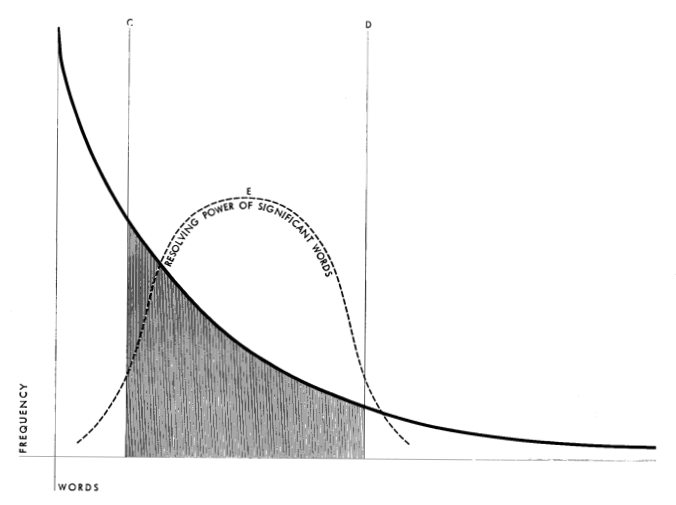
\includegraphics[scale=0.8]{Luhn58Phot.png}
\captionof{figure}{Diagramme des fréquences des mots et le choix de Luhn \cite{Luhn58}}\label{Luhn58Phot}
\end{center}
\end{itemize}
Cette approche, comme on l'a mentionné au début, est assez moins précise et empirique, mais elle sous-tend les idées fondamentales appliquées plus tard.

\subsubsection{Algorithme TF-IDF}\label{SousSecTFIDF}
$ _{} $ $ _{} $ $ _{} $ $ _{} $ $ _{} $Le \textit{\textbf{tf-idf}} (\textit{time-frequency inverse document frequency}) est une approche essentiellement utilisée pour le résumé extractif. Il s'agit d'une correction de l'approche naïve consistant à poser que plus un mot est répété dans un corpus de texte, plus il y est important.\\

Soit donc un corpus constitué de $ D $ documents et $ N_{j} $ le nombre total de mots (termes) présents dans un document $ j $ donné du corpus. Nommons $ Freq(i,j) $ le nombre de fois qu'un terme $ i $ apparaît dans le document $ j $.\\
On définit classiquement la fréquence d'apparition par :
\begin{eqnarray}
TF(i,j) = \frac{Freq(i,j)}{N_{j}}
\end{eqnarray}
L'approche qui se base naïvement sur la fréquence d'apparition des mots dans les textes pour juger de leur importance relative, accorde à chaque mot un poids égal à $ TF(i,j) $.\\
La grande faiblesse de cette approche est d'inclure ainsi des termes sans grande pertinence in\-for\-ma\-tion\-ne\-lle comme des prépositions, des articles,... très présents au sein des documents.\\

Pour corriger cette faiblesse, on pose l'hypothèse que les termes importants apparaissent plusieurs fois dans un document (ou juste dans peu de documents du corpus) et non pas dans plusieurs documents, puisque dans le cas où c'est dans plusieurs documents, il est souvent question des éléments communs du langage, sans grande utilité informationnelle. Ceci constitue en fait \textit{la loi de Zipt} \cite{vzivzka2019text} et c'est le fondement de l'approche du \textit{tf-idf}.\\

A cet effet, on définit $ DF_{i} $ comme étant le nombre de documents dans le corpus, qui contiennent le terme numéro $ i $. Cela permet d'affecter alors le poids selon la formule \cite{berry2010text} :
\begin{eqnarray}\label{Tf-Idf-Formula}
TFIDF(i,j) = \log\left(1+TF(i,j)\right)\cdot\log\left(\frac{D}{DF_{i}}\right)
\end{eqnarray}
Dans l'expression \ref{Tf-Idf-Formula}, en supposant que $ N $ est le dictionnaire des termes présents dans l'ensemble des documents et $ D $ le nombre de documents du corpus, il faut noter que :\\
$ i \in \left\lbrace 1,...,N\right\rbrace $ et $ j \in \left\lbrace 1,...,D\right\rbrace $.\\

D'où finalement, le poids d'un terme $ i $ dans un document $ j $ est donné par :
\begin{eqnarray}
w_{ij} = TFIDF(i,j)
\end{eqnarray}
Pour notre cas, l'application de cette approche consiste à décomposer un long texte en ses phrases et de considérer que chacune de ces phrases est un document et que le texte entier constitue le corpus.\\

Plusieurs définitions des éléments $ TF(ij) $ et $ IDF_{i} $ formant l'expression \ref{Tf-Idf-Formula} sont toutefois possibles selon les besoins en terme  de performance.\\
Mais, dans l'ensemble, l'idée de base demeure la même car il ne s'agit en général que de changement des types de normalisation \cite{vzivzka2019text}.\\

L'application de cette méthode pour le résumé consiste fi\-na\-le\-ment à calculer le poids de chaque phrase en additionnant les poids des termes la constituant, puis à normaliser le résultat en fonction de la taille de la phrase considérée. Après tout, on définit un seuil qui permet de soutirer les phrases selon leur pertinence ainsi évaluée (en considérant évidemment plus pertinente une phrase dont le résultat de la sommation des poids est élevé).
\subsubsection{Algorithme TextRank}
\textit{TextRank} est un algorithme de résumé extractif, basé sur la théorie des graphes et qui s'inspire de l'algorithme \textit{PageRank} de Google \cite{brin1998anatomy,benincasa2006page}.\\
A la base, on considère un ensemble de $ N $ phrases donné, et on calcule les coefficients de liaison de chaque phrase aux $ N-1 $ autres. A la fin, on peut obtenir une matrice $ M $ de taille $ N\times N $ dont chaque terme $ M_{ij} $ représente le degré de liaison entre la phrase numéro $ i $ et la numéro $ j $. Il s'agit en fait d'une \textit{matrice d'adjacence} dans laquelle on pose au préalable que $ M_{ii} = 0 \mbox{, pour tout } i $ (c'est la même idée pour l'algorithme \textit{PageRank} étant donné qu'il est logique de considérer qu'une page ne peut s'auto-référencer).\\

Soit donc $ i \in \left\lbrace 1,..., N \right\rbrace $. Appelons $ Phr_{i} $ la phrase numéro $ i $ du corpus. Cela veut dire qu'on peut écrire :
\begin{eqnarray}
Liaison \mbox{ } Phr_{i}\leftrightsquigarrow Phr_{j} = M_{ij} = M_{ji}
\end{eqnarray}
Les valeurs de $ M_{ij} $ sont calculées au choix, selon le programmeur. Ce dernier implémente en effet une mesure de similarité selon sa définition de la liaison entre phrases et les besoins en performance.\\
C'est ainsi qu'on peut utiliser par exemple une mesure de similarité classique nommée \textit{similarité cosinus} en la basant par exemple sur $ TFIDF $ \cite{COSINindurkhya2010handbook}.\\
Pour représenter les mots à comparer, on utilise les méthodes classiques de vectorisation des mots (\textit{word embedding}). Nous esquisserons ces méthodes dans les sections qui vont suivre, parlant du \textit{word embedding} ( \ref{SectionSeq2Seq} ).\\

Le rang des phrases sont alors calculés de manière itérative en s'inspirant de la formule \cite{mihalcea2004textrank} :
\begin{eqnarray}\label{TextR-Formula}
TextRank\left(Phr_{i}\right) = (1-K)+K\cdot \sum\limits_{\underset{j \neq i}{j=1}}^N \left[TextRank(Phr_{j})\right]\cdot M_{ij}
\end{eqnarray}
Dans cette formule, $ K $ est une constante comprise entre $ 0 $ et $ 1 $.\\
Initialement, on prend en général une valeur identique de $ TextRank(Phr_{i}) $ pour toutes les phrases (souvent $ TextRank(Phr_{i})=1 $), mais la valeur initiale prise n'affecte pas les valeurs finales, mais elle affecte le temps de convergence \cite{mihalcea2004textrank}.\\

La formule \ref{TextR-Formula} n'est pas arbitraire, elle est d'ailleurs triviale si on s'inspire de l'algorithme de \textit{PagePank} la plus simple. Pour cet algorithme (\textit{PageRank}), on avait pris à l'origine $ K=0.85 $ \cite{brin1998anatomy}.\\
\paragraph{\underline{Justification de la formule}}
Le principe de \textit{PageRank} consiste à se dire que, si une page $ Pag_{i} $ contient $ N_{i} $ références vers d'autres pages, la probabilité qu'on aille vers l'une de ces pages référencées est de $ \frac{1}{N_{i}} $ (avec l'hypothèse que les références ne sont pas répétées et que la distribution de leur importance est uniforme). On sait tout de même que plus une page est référencée, plus on doit lui donner de l'importance.\\
Si alors on pose que l'importance de la page $ Pag_{i} $ est connue, le calcul de l'importance d'une page $ Pag_{j} $ vers laquelle elle pointe se calculera logiquement par :
\begin{eqnarray}\label{PageRankBEGIN}
Importance(Pag_{j}) = \sum_{i} Importance(Pag_{i})\cdot \frac{1}{N_{i}}
\end{eqnarray}
Avec $ i $ appartenant à l'ensemble des pages qui mentionnent la page $ Pag_{j} $ en leur sein.\\
Malheureusement, pour les phrases non référencées (pages dites isolées), on trouve une importance nulle. Pour lutter contre cela, la formule \ref{PageRankBEGIN} est un peu modifiée en y introduisant adéquatement une constante non nulle $ K $.\\
Ce qui donne l'expression \cite{brin1998anatomy} :
\begin{eqnarray}\label{PageRank}
Importance(Pag_{j}) =(1-K) + K\cdot\sum_{i} Importance(Pag_{i})\cdot \frac{1}{N_{i}}
\end{eqnarray}
On voit alors qu'il s'agit belle et bien de la formule utilisée pour \textit{TextRank} (formule \ref{TextR-Formula}).\\

Après initialisation des rangs de chaque phrase du texte ( les $ TextRank(Phr_{i}) $) et après calcul de la matrice d'adjacence $ M $. On applique la formule \ref{TextR-Formula} itérativement et à la convergence, on choisit les phrases qui vont former le résumé selon leur importance ( valeurs des $ TextRank(Phr_{i}) \mbox{ pour toute valeur de } i $).\\
A la fin, les phrases sélectionnées sont réarrangées pour former un résumé extrait plus ou moins cohérent.\\

Il existe également un algorithme nommé \textit{\textbf{LexRank}} \cite{erkan2004lexrank} qui est assez similaire à \textit{TextRank} ici décrit, à la différence près que :
\begin{itemize}
\item[-] Il prend essentiellement en compte les métriques de similarité robustes;
\item[-] Il considère la position et la longueur des phrases dans le calcul de leur pertinence;
\item[-] Il est optimisé pour le résumé multi-document.
\end{itemize}

Plusieurs autres algorithmes populaires existent, par exemple les algorithmes \textit{\textbf{LSA}} (\textit{Latent Semantic Analysis} ou Analyse Sémantique Latente) et \textit{\textbf{LDA}} (\textit{Latent Dirichlet Allocation} ou Allocation Latente de Dirichlet) \cite{berry2010text}.\\
Le premier, la \textit{LSA}, est un algorithme statistique, basé sur l'algorithme \textit{\textbf{SVD}} (\textit{Singular Value Decomposition} ou décomposition en valeurs singulières). Seulement, cette technique est très gourmande en ressources suite à la complexité de l'algorithme qui implémente le \textit{SVD}. Le second, la \textit{LDA}, basé sur la détection des thématiques, peut aussi être utilisé.\\

Toutefois, il faut remarquer que les algorithmes ici présentés sont essentiellement adaptés à la synthèse extractive. Même si ces traitements peuvent être mélangés avec les \textbf{techniques de résolution d'anaphores} et les \textbf{paraphrases} pour obtenir des synthèses qui tendent vers la synthèse abstractive, nous devons souligner que les techniques jusque là les plus performantes pour la synthèse abstractive sont essentiellement basées sur le \textit{deep learning} \cite{MaaliMnasri}. Le \textit{deep learning} peut également être utilisé pour la synthèse extractive, permettant ainsi la génération des synthèses extraites plus cohérentes (avec résolution d'anaphores). Ainsi donc, nous abordons les méthodes de \textit{deep learning} utilisées pour cet effet dans les parties qui suivent.
\section{Modèles Seq2Seq}\label{SectionSeq2Seq}
\subsection{Methodes du Word-Embedding}
$ _{} $ $ _{} $ $ _{} $ $ _{} $ $ _{} $Tout traitement commence par une représentation numérique des termes (des mots ici) pour qu'ils soient assimilables par le modèle. Une approche naïve consisterait à regrouper tous les mots de notre vocabulaire dans une liste (un dictionnaire) et de les représenter chacun par un nombre unique (un identifiant). Une autre approche, plus classique, consiste à représenter chaque mot par un vecteur de dimension égale à la taille du dictionnaire et dont tous les termes sont nuls, sauf à la position, dans le dictionnaire, du mot qu'on est entrain de vouloir représenter (on parle du \textit{one-hot encoding}).\\
$ _{} $ $ _{} $ $ _{} $ $ _{} $ $ _{} $Ces représentations, et toutes celles qui s'y apparentent, ont la grande faiblesse d'être peu  informatives (au point de vu sémantique). Étant artificiellement construites, sans tenir compte du sens des mots, ni de leur contexte, ces méthodes de représentation rendent la tâche de découverte des caractéristiques par les systèmes de \textit{machine learning} encore plus difficile. D'ailleurs, l'une des faiblesses de la seconde méthode décrite (le \textit{one-hot encoding}) est que les vecteurs sont creux (une majorité de valeurs nulles) et de dimension inutilement très grande. On pourrait directement songer à une représentation plus ju\-di\-cieu\-se pour éviter ces deux soucis, et qui consisterait à réaliser une représentation binaire des termes mais, le problème de la sémantique sera toujours là.\\
$ _{} $ $ _{} $ $ _{} $ $ _{} $ $ _{} $On recourt donc à des méthodes de représentation plus élaborées, partant du principe selon lequel le contexte d'un mot suffit pour en appréhender le sens. Ainsi, tout mot est représenté en réalisant une statistique (implicitement bien sûr) sur les divers mots qui l'accompagnent souvent, de telle sorte que les mots aux sens proches aient aussi des vecteurs très proches. Bref, on en arrive à réaliser la proposition : "Similarité sémantique implique similarité de représentation". Ce sont les méthodes classiques du \textit{word embedding} (ou plongement lexical). Il s'agit par exemple des méthodes comme le \textit{\textbf{Word2Vec}} \cite{WORD2VECmikolov2013efficient, WORD2VEC2mikolov2013distributed}, \textit{\textbf{Glove}} \cite{GLOVEpennington2014glove}, \textit{\textbf{fastText}} \cite{FASTtEXTbojanowski2017enriching}...\\

\subsection{Modèles séquence-à-séquence proprement dits}
$ _{} $ $ _{} $ $ _{} $ $ _{} $ $ _{} $S'agissant des modèles séquence-à-séquence (\textit{Seq2Seq}), ils ont été présentés dans la section \ref{AttentionEtseq2seq} (voir particulièrement la figure \ref{FigureSeq2Seq}). Il s'agit bel et bien des modèles adaptés aux tâches de synthèse, vu qu'en entrée on reçoit une séquence pour ressortir une autre séquence en sortie.\\
Comme nous l'avons déjà bien mentionné au précédent chapitre, nous n'allons parler que des modèles \textit{Seq2Seq} de type \textit{transformer} car actuellement, ils sont les plus adaptés à la tâche que nous voulons réaliser (celle de synthèse automatique). Les \textit{transformers} (voir la figure \ref{ImgTransformerVASWANI}) sont un modèle très avantageux car en fait, au-delà de leurs performances et autres avantages, ils facilitent encore plus la recherche en \textit{NLP} en rendant effectif le \textit{transfer learning} (apprentissage par transfert) dans ce domaine.\\

L'entraînement des \textit{transformers} est \textit{semi-supervisé}. Il se fait en deux crans (nous les décrirons dans le cadre du \textit{NLP}) :
\begin{itemize}
\item[1°)] \textit{\textbf{Pré-entraînement}} : il s'agit d'un \textit{apprentissage non supervisé}, qui consiste à donner au modèle une masse colossale de données textuelles, non étiquetées, pour qu'il développe une compréhension statistique du langage qu'on veut qu'il puisse assimiler. Au final, on obtient un modèle pré-entraîné.
\item[2°)] \textit{\textbf{Affinage de l'apprentissage}} (\textit{fine-tuning}) : Ça consiste à finaliser l'apprentissage du modèle pré-entraîné \textit{de manière supervisée} pour qu'il soit en mesure de réaliser une tâche donnée du \textit{NLP} (il s'agit du \textit{transfer learning} en fait). Cette spécialisation, requiert une très faible quantité de données car le modèle aura déjà une représentation assez bonne de la langue. Cela pallie à la fois au problème de manque des données labellisées en \textit{NLP} et de la consommation en terme de ressource énergétique des gros modèles lors de leur entraînement. 
\end{itemize}
Les méthodes de pré-entraînement sont très déterminantes pour les performances finales du modèle. Ce premier entraînement du modèle a pour rôle de l'amener à construire un \textit{\textbf{modèle de langage}} \cite{BART}.\\
Il existe ainsi plusieurs objectifs de de pré-entraînement (pour construire le modèle de langue). On peut par exemple entraîner le modèle à :
\begin{itemize}
\item[-] Prédire le mot suivant : donc, lors de cet entraînement non supervisé, on fournit chaque fois au modèle une séquence de mots en lui demandant de prédire le suivant. Il s'agit d'un objectif d'entraînement dit \textit{NSP} (\textit{Next Sentence Prediction}) visant à transformer implicitement le \textit{transformer} en un modèle de langue  \cite{BERT_devlin2018bert};
\item[-] Deviner le mot caché (masqué) : on fournit au modèle du texte dont certaines parties (mots ou suite de mots) sont cachées. L'objectif assigné au modèle est alors de retrouver les mots masqués. On parle du \textit{MML} (\textit{Masked Language Modelling}) \cite{BERT_devlin2018bert}.
\end{itemize}
Ainsi, au fur et à mesure, les paramètres du modèle s'affinent, le transformant en un modèle de langue performant. Mais, à part les deux que nous venons de mentionner, il existe d'autres \textit{objectifs de pré-entraînement} \cite{BART,PEGASUSzhang2020pegasus} selon les variantes de \textit{transformers} et les objectifs finaux de spécialisation du modèle.\\

Bien que la forme classique des \textit{transformers} est bel et bien celle de la figure \ref{ImgTransformerVASWANI}, il existe $ 3 $ types d'implémentation selon les types de tâche visées en dernier lieu :
\begin{itemize}
\item[1°)] Modèles à encodeur seul : on supprime la partie décodeur. Ces modèles sont très bons pour les tâches de compréhension du langage comme la classification par exemple.
\item[2°)] Modèles à décodeur seul : on supprime alors la partie décodeur du modèle. Ils sont bons pour les tâches de génération de texte.
\item[3°)] Modèles encodeur-décodeur : ou encore modèles \textit{seq2seq} proprement-dits. Ils sont bons pour les tâches demandant à la fois la compréhension et la génération des textes.
\end{itemize}
Pour illustrer ce fait, on va considérer donc $ 3 $ types de \textit{transformers} \cite{GRAAL_HF_tunstall2022natural, HF_wolf2020transformers} :
\begin{itemize}
\item[1°)] \textit{Like-BERT} : semblables au transformer dénommé \textit{BERT} (\textit{Bidirectional Encoder Re\-pre\-sen\-ta\-tions from Transformers}). Ce sont des modèles du type encodeur seul. Ils sont également bidirectionnels. Donc, les phrases sont lues dans les deux sens pour mieux saisir tout le contexte.
\item[2°)] \textit{Like-GPT} : donc semblables au \textit{transformer} dénommé \textit{GPT} (\textit{Generative Pre-trained Transformer}) qui n'ont que la partie décodeur et sont dits \textit{auto-regressifs} car, seules les parties précédant le mot en cours de traitement sont connues du modèle et il y a chaque fois réinjection des sorties à l'entrée.
\item[3°] \textit{Like-BART/T5} : semblables à \textit{BART} (\textit{Bidirectional and Auto-Regressive Transformers}) ou à  \textit{T5} (\textit{Text-To-Text Transfer Transformer}). C'est donc ceux du type encodeur-décodeur.
\end{itemize}
\paragraph{\underline{Modèles encodeurs (\textit{encoder-model})} :} Comme on l'a dit, pour ces modèles, on n'imp\-lé\-men\-te que la partie encodeur du \textit{transformer} d'origine (celui d'origine étant dans \cite{vaswani2017attention}). En plus de cela, ces modèles ont une couche d'attention bidirectionnelle et sont généralement appelés \textit{auto-encodeurs} (\textit{auto-encoding model}). Ces modèles sont principalement bons pour les tâches de \textit{NLU} (\textit{Natural Language Understanding}) comme la classification, le \textit{NER} (\textit{Name Entity Recognition}), l'\textit{extractive question-answering},...\\
Dans ce groupe, les modèles les plus connus sont :
\begin{itemize}
\item[•] ALBERT \cite{lan2019albert},
\item[•] BERT \cite{BERT_devlin2018bert},
\item[•] DistilBERT \cite{sanh2019distilbert},
\item[•] RoBERTA \cite{liu2019roberta},
\item[•] Etc.
\end{itemize}

\paragraph{\underline{Modèles décodeurs (\textit{decoder-models})} :}
Utilisent seulement la partie décodeur, sont auto-regressifs et par conséquent les têtes de \textit{self-attention} n'accèdent qu'aux mots précédant l'étape à laquelle elles sont (pas de regard dans le futur) comme on l'a déjà un peu mentionné. Ces modèles sont particulièrement bons pour les tâches liées fortement au \textit{NLG} (\textit{Natural Language Generation}).\\
Dans ce groupe, les modèles les plus connus sont :
\begin{itemize}
\item[•] Les GPT ($ 1 $, $ 2 $ et $ 3 $) \cite{GPT2_radford2019language},
\item[•] TransformerXL \cite{dai2019transformer},
\item[•] Etc.
\end{itemize}

\paragraph{\underline{Modèles encodeur-décodeur (\textit{sequence-to-sequence models})} :}
Ces modèles utilisent l'in\-té\-gra\-li\-té de l'architecture des \textit{transformers} et sont ainsi bons pour les tâches demandant à la fois du  \textit{NLU} et du \textit{NLG} comme la synthèse automatique abstractive, le \textit{generative question-answering} et la traduction automatique.\\
Ici nous pouvons particulièrement mentionner les modèles comme :
\begin{itemize}
\item[•] BART \cite{BART},
\item[•] mBART \cite{mBART_liu2020multilingual},
\item[•] BARThez \cite{eddine2020barthez},
\item[•] T5 \cite{T5-raffel2020exploring},
\item[•] mT5 \cite{mT5_xue2020mt5},
\item[•] PEGASUS \cite{PEGASUSzhang2020pegasus},
\item[•] Etc.
\end{itemize}

\subsection{Modèle BART pour la synthèse abstractive}\label{BARTmodel}
Le modèle \textit{BART} est comme une combinaison de \textit{BERT} \cite{BERT_devlin2018bert} et de \textit{GPT-2} \cite{GPT1_radford2018improving,GPT2_radford2019language} en terme d'architecture et d'objectif de pré-entraînement, avec quelques optimisations supplémentaires \cite{BART}.
Pour illustration, voici une image de comparaison :
\begin{center}
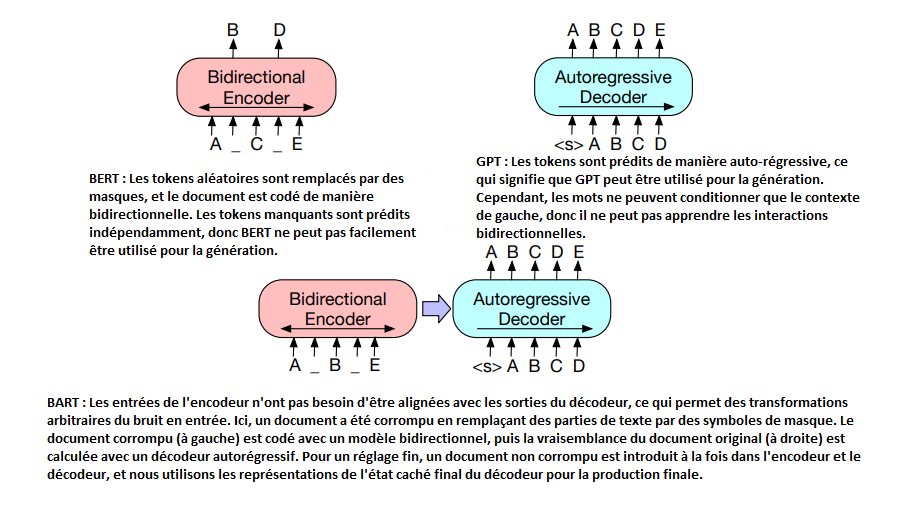
\includegraphics[width=15cm]{GPT_BERT_BART.png}
\captionof{figure}{Comparaison simplifiée entre BERT, GPT et BART \cite{BART}}\label{ComparisonBART}
\end{center}
$ _{ } $\\
L'image \ref{ComparisonBART} étant claire, nous pouvons illustrer les diverses corruptions que peuvent subir les données pour le pré-entraînement. L'image ci-dessous l'illustre :\newpage
\begin{center}
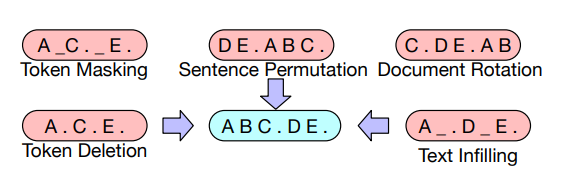
\includegraphics[scale=1]{TransForNOISING.png}
\captionof{figure}{Transformations de bruitage expérimentées pour BART \cite{BART}}
\end{center}
Le modèle \textit{BART} est bien adapté à la tâche de synthèse abstractive. C'est celui que nous allons utiliser (les modèles dérivés de \textit{BART} principalement) pour réaliser cette tâche dans notre système.
\subsubsection{Justification du choix de BART}
$ _{} $ $ _{} $ $ _{} $ $ _{} $ $ _{} $Le choix de \textit{BART} est dû au fait que c'est le modèle que nous avons trouvé réalisant un bon compromis poids-performances. Aussi, après quelques tests, ses résultats nous ont paru être plus intéressants. En outre, l'objectif d'entraînement utilisé pour \textit{BART} nous paraît assez général pour construire un modèle de langage performant. Nous justifierons plus précisément ce choix dans le chapitre qui suit, en présentant également quelques résultats des tests.
\section{Conception de l'architecture globale de \textit{Mon Résumeur}}
$ _{} $ $ _{} $ $ _{} $ $ _{} $ $ _{} $Il existe un large éventail des méthodes de développement des systèmes informatiques mais, en règle générale, toutes suivent les étapes suivantes \cite{CoursGenieLogiciel} :
\begin{itemize}
\item[1°)] Spécifications : on définit avec précision ce que fera le système (à quoi est-il destiné?);
\item[2°)] Conception et mise en oeuvre : on conçoit et on réalise le système;
\item[3°)] Validation : on teste le système pour voir s'il correspond aux objectifs précisés dans les spécifications;
\item[4°)] Évolution : ça correspond à tout ce qui vient après la livraison du produit (\textit{versionning}, maintenances,...).
\end{itemize}
Ici, on ne va pas utiliser une méthode de conception particulière. Pour pouvoir tout de même y aller méthodiquement, nous nous inspirerons de ces étapes classiquement suivies lors de la conception des systèmes informatiques.\\
Dans ce second chapitre, nous ne présenterons que les spécifications du système ainsi qu'une ébauche de conception avec une présentation de l'architecture globale. La suite sera traitée dans le chapitre suivant.
\subsection{Spécifications du système}
$ _{} $ $ _{} $ $ _{} $ $ _{} $ $ _{} $Le système devra pouvoir permettre de réaliser ce qui suit :
\begin{itemize}
\item[-] Synthétiser les textes qui lui sont fournis en entrée (saisis directement ou importés dans fichiers \textit{.pdf} non scannés, des fichiers \textit{.docx} et \textit{.txt});
\item[-] Servir les synthèses directement ou à travers un fichier \textit{.pdf} à télécharger;
\item[-] Obtenir des synthèses produites par plusieurs algorithmes et les évaluer;
\item[-] Stocker les couples document-synthèse;
\item[-] Permettre l'affinage d'un modèle de synthèse automatique (ici nous réaliserons le \textit{fine-tuning} du modèle \textit{mBART} ou du modèle \textit{mT5} selon celui qui se prêtera mieux à cet affinage).
\end{itemize}
C'est cela le minimum de besoins que le système devra être capable de combler.
\subsubsection{Exigences fonctionnelles}
Pour fonctionner, nous allons considérer que les fichiers chargés (pour en obtenir le résumé) seront au format \textit{pdf}, \textit{txt} ou \textit{docx} et qu'ils seront en français.
\subsubsection{Exigences non fonctionnelles}
Comme exigence non fonctionnelle, on doit noter qu'un processus d'authentification sera utile, songeant à une rentabilisation future du système.
\subsection{Présentation des éléments du système}
$ _{} $ $ _{} $ $ _{} $ $ _{} $ $ _{} $L'architecture globale de notre système est un trois-tiers classique. Elle se présentera comme sur la figure \ref{ArchiSysteme}:
\begin{center}
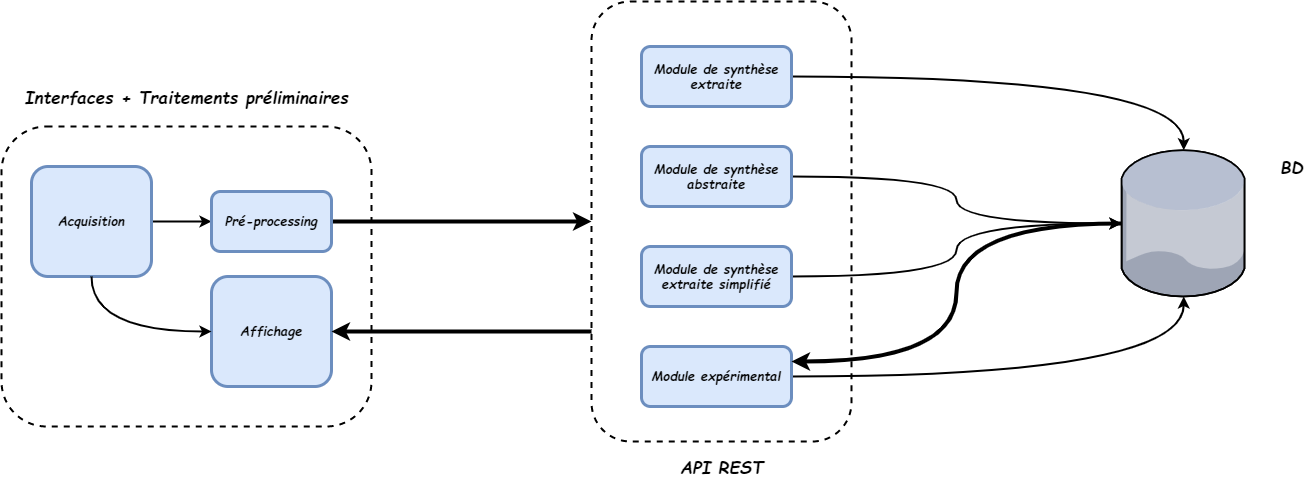
\includegraphics[width=16cm]{ArchiSysteme.png}
\captionof{figure}{Architecture globale de notre système}\label{ArchiSysteme}
\end{center}
La figure \ref{ArchiSysteme} présente l'architecture du système qui est une architecture $ 3-tiers $ classique. Il y a toutefois une partie qui n'est pas ici représentée car nous voulons nous donner une grande liberté de conception à son sujet. Il s'agit en fait de l'interface d'accès à l'\textit{API} (\textit{Application Programming Interface}), qui permettra aux développeurs de s'authentifier et générer éventuellement un \textit{token} à utiliser pour implémenter leurs propres interfaces devant permettre d'utiliser les services de cette \textit{API}. Il s'agit donc d'une \textit{API privée}.\\
Cette interface permettra aussi de voir toute la documentation de l'\textit{API} (pour les dé\-ve\-lop\-peurs) pour mieux utiliser ses services.

Quant au bloc interface que nous venons de présenter sur la figure \ref{ArchiSysteme}, c'est en nous mettant à la place d'un développeur lambda qui exploite les services de l'\textit{API}.\\
$ _{} $ $ _{} $ $ _{} $ $ _{} $ $ _{} $Notre \textit{API} quant à elle, est une \textit{API} \textit{REST} (\textit{REpresentationnal State Transfer}) qui aura $ 4 $ \textit{end-points} principaux dédiés à la synthèse automatique (selon les besoins d'imp\-lé\-men\-ta\-tion, on pourra en insérer d'autres mais qui ne concernerons probablement pas la synthèse).
\begin{itemize}
\item[•] \textit{Module de synthèse extraite} : ce module réalisera une synthèse en combinant divers résultats d'algorithmes de synthèse extraite. Nous prévoyons, dans un premier temps, ne l'utiliser que pour des petits documents (la taille optimale sera déterminée avec les expérimentations au chapitre suivant).
\item[•] \textit{Module de synthèse abstraite} : ce module donnera une synthèse abstraite en utilisant l'un des \textit{transformers} affinés pour la synthèse ou bien par le module qui sera en train d'être amélioré au cours de l'utilisation du système (on l'a nommé \textit{expérimental} sur les interfaces, voir la figure \ref{EbaucheInterface}). Comme les \textit{transformers} réalisent des synthèses de documents de taille généralement limitée à environ une page, nous mettrons au point, dans cette partie, un pipeline qui nous permettra d'augmenter le nombre de pages (nous pensons à $ 100 $ pages mais les expérimentations nous permettrons de choisir une taille optimale, tenant compte surtout de la rapidité). Le pipeline en question peut se résumer par la figure \ref{PipelineSumm} qui suit :
\begin{center}
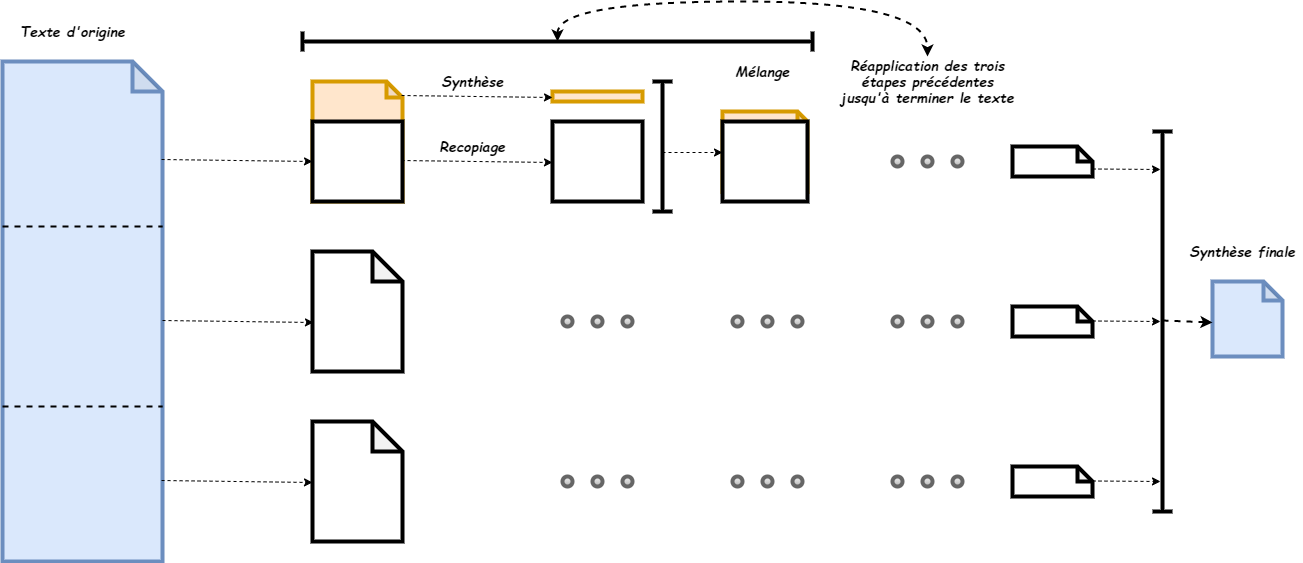
\includegraphics[width=16.5cm]{PipelineSummary.png}
\captionof{figure}{Pipeline de synthèse abstractive}\label{PipelineSumm}
\end{center}
$ _{} $ $ _{} $ $ _{} $ $ _{} $ $ _{} $Sur la figure \ref{PipelineSumm}, la particularité réside au fait que dans l'implémentation, les divisions se feront en découpant au préalable tout texte en ses phrases constitutives, puis, en reliant un certain nombre de phrases se présentant en tête de chaque partie jusqu'à atteindre une longueur inférieure à la limite admissible par le modèle utilisé. Finalement, la synthèse obtenue pour cette sous-partie sera ajoutée à la partie globale et le processus se répétera comme l'illustre la figure. Nous avons testé cette méthode et elle nous a permis de mieux conforter le compromis vitesse-qualité par rapport aux pipelines classiques \cite{GRAAL_HF_tunstall2022natural}.
\item[•] \textit{Module de synthèse extrait simplifié} : Il s'agira d'un module qui permettra la réalisation de la synthèse mais en utilisant l'un des algorithmes de synthèse extraite (le plus rapide).
\item[•] \textit{Module expérimental} : Il s'agira d'un module de synthèse abstraite qui sera es\-sen\-tiel\-le\-ment utilisé pour la synthèse des petits documents (quelques pages). Ce module sera entraîné à partir des synthèses collectées par le système, pour améliorer au fur et à mesure ses performances. Nous comptons réaliser l'entraînement par \textit{transfer learning} avec le \textit{transformer} \textit{mBART} \cite{mBART_liu2020multilingual} comme base. 
\end{itemize}
On peut aussi remarquer qu'il y a un module \textit{pre-processing} dans la partie interfaces. C'est à la suite du fait que, pour des raisons de performance, on devra envoyer à l'\textit{API} le fichier sous un format particulier. Il faudra réaliser l'acquisition des données dans divers formats (\textit{pdf},\textit{docx},...) mais les données acquises seront envoyées dans un format plus léger à l'\textit{API} (du \textit{JSON} pour notre cas). \textbf{Ce \textit{pre-processing} consistera donc à extraire les données des documents fournis en entrée. Cela devra être fait sans les corrompre pour s'assurer de la qualité des résumés.}\\
$ _{} $ $ _{} $ $ _{} $ $ _{} $ $ _{} $La base des données, que nous avons mentionné dans la figure \ref{ArchiSysteme} a un double rôle :
\begin{itemize}
\item[1°)] Le stockage des données de l'utilisateur (il s'agira en fait des identifiants des in\-ter\-fa\-ces qui utiliseront l'\textit{API});
\item[2°)] Le stockage des paires document-synthèse, ainsi que l'appréciation de l'utilisateur (évaluation par les utilisateurs).
\end{itemize}
\subsection{Architecture du module de synthèse extractive}\label{SectionMerging}
$ _{} $ $ _{} $ $ _{} $ $ _{} $ $ _{} $Le module de synthèse extractive, que nous nommerons \textit{\textbf{merging}}, se présente comme suit :\newpage
$ _{ } $\\
\begin{center}
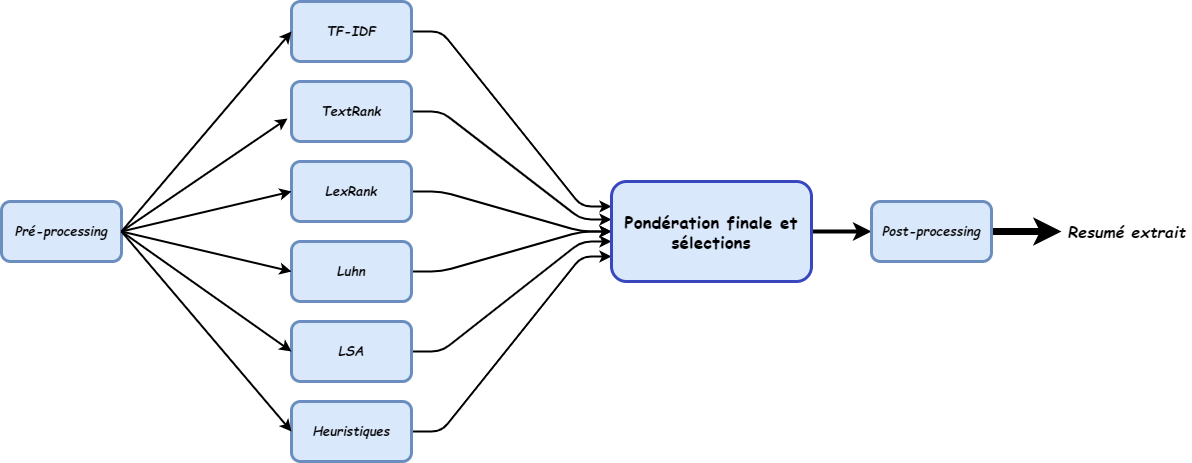
\includegraphics[width=16cm]{ResumeExtrait.png}
\captionof{figure}{Architecture globale du module de synthèse extractive}\label{ArchiGlobExtract}
\end{center}
$ _{ } $\\
Comme nous pouvons le voir sur la figure \ref{ArchiGlobExtract}, un traitement sera fait pour adapter les données reçues à ce qui peut être traité par le système. Ce traitement consistera es\-sen\-tiel\-le\-ment à réaliser la \textit{tokenisation} des textes (chaque \textit{token} sera une phrase pour cette partie) et à affecter un identifiant unique à chaque phrase.\\
Après cela, les données seront invariablement passées aux divers algorithmes de synthèse ex\-tra\-ctive (\textit{TFIDF, LexRank, ...}), qui générerons chacun un groupe de poids des phrases. Après cela, le module de pon\-dé\-ra\-tion et sélection réalisera successivement ce qui suit :
\begin{itemize}
\item[1°)] Acquisition des sorties de chaque algorithme de synthèse extractive (il s'agira des dictionnaires dont les clés seront les identifiant uniques des phrases et les valeurs seront les poids affectés par l'algorithme). A chaque algorithme, on donnera un poids qu'on nommera $ W_{Nom de l'algo} $ compris entre $ 0 $ et $ 1 $, selon la confiance qu'on lui porte (la somme des poids sera égale à $ 1 $ et par défaut, tous les algorithmes pourront avoir le même poids) ;
\item[2°)] Élimination des phrases de poids faible (avec comme seuil, la taille maximale de résumé précisée par l'utilisateur) ;
\item[3°)] Réarrangement de chaque dictionnaire obtenu après expulsion des phrases non si\-gni\-fi\-ca\-ti\-ves (les éléments seront arrangés par ordre décroissant des poids pour chaque sortie);
\item[4°)] Donner des probabilités aux espaces des poids de chaque dictionnaire par application d'un \textit{softmax} sur chacun d'eux. Ce qui donnera, pour chaque phrase de chaque dictionnaire, un nouveau poids $ \omega_{phr_{i}} $, avec $ i $ le numéro du dictionnaire et $ phr $ le numéro de la phrase considérée dans ce dictionnaire ;
\item[5°)] Listage complet des éléments (leurs identifiants) de tous les dictionnaires.
\item[6°)] Pour chaque élément de la liste globale ainsi établie, appliquer la formule suivante pour obtenir un nouveau poids :
\begin{eqnarray}
\mathcal{W}_{j} = \sum_{i\in \mathcal{D}}\left( W_{i}\cdot \omega_{phr_{i}}\right)
\end{eqnarray}
Avec $ \mathcal{W}_{j} $ le nouveau poids affecté à la phrase ayant un identifiant global $ j $ (l'identifiant là d'origine) et $ \mathcal{D} $ la liste des dictionnaires (les sorties de chaque algorithme) ;
\item[7°)] Arranger toutes les phrases par ordre décroissant dans une unique liste et sélectionner les plus haut dans la liste jusqu'à atteindre le seuil fixé (nombre de mots fixé pour la synthèse).
\item[8°)] Constituer une liste avec les éléments sélectionnés.
\item[9°)] Réarranger les phrases de la liste selon leur ordre de succession dans le texte d'origine.
\item[10°)] Constituer la synthèse extraite.
\end{itemize}
Ce qui précède constitue en fait l'algorithme que nous allons implémenter pour le \textit{module de pondération et sélection}. Précisons seu\-le\-ment que, les poids des algorithmes (voir le paramètre $ W_{Nom de l'algo} $ du point $ 1° $ de la description ci-dessus) seront accordés de manière statique et non dynamique. Pour les choisir, nous allons nous servir des scores de chacun de ces algorithmes aux diverses métriques que nous présenterons au chapitre suivant. Et c'est à cette même occasion que nous préciserons les valeurs choisies pour ces paramètres ( Valeurs à retrouver dans le tableau \ref{MergingWeights}).
\subsection{Architecture du module de synthèse abstractive}
$ _{} $ $ _{} $ $ _{} $ $ _{} $ $ _{} $Le module de synthèse abstraite n'est pas unique. Nous implémenterons plusieurs modèles (\textit{BART}, \textit{BARThez}, \textit{PEGASUS} et \textit{mBART} entraîné avec nos données); Chaque module de synthèse se présentera néanmoins comme suit :
$ _{ } $\\
\begin{center}
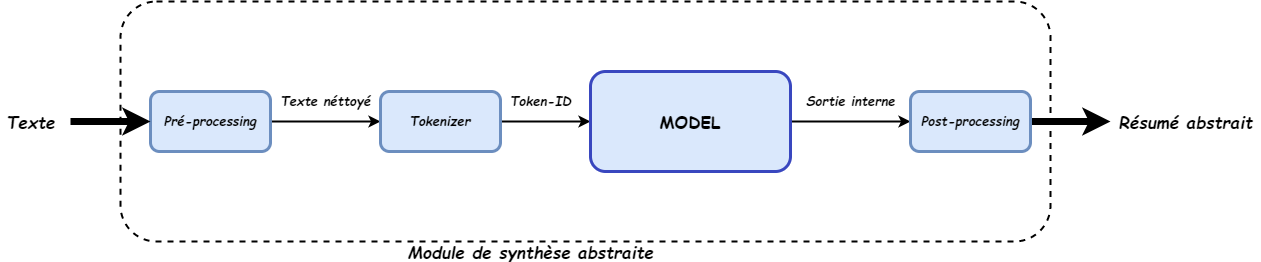
\includegraphics[width=16cm]{ResumeAbstraitGLOBAL.png}
\captionof{figure}{Architecture globale du système de synthèse abstractive}\label{ArchiGloAbstract}
\end{center}
$ _{ } $\\
Comme nous pouvons le remarquer, il y a toujours un module de mise en forme initial (\textit{pre-processing}) qui nous permettra en gros de supprimer tous les caractères que nous ne pourrons pas gérer. Vient ensuite le module de tokenisation (le \textit{tokenizer} ou tokeniseur) \cite{GRAAL_HF_tunstall2022natural}  qui consistera ici à diviser tout le texte en ses mots constitutifs et à leur affecter des identifiants numériques. Ce sont ces identifiants qui seront fournis au modèle et transformés en vecteurs par la couche d'\textit{embedding} du modèle.\\
$ _{} $ $ _{} $ $ _{} $ $ _{} $ $ _{} $Le modèle quant à lui, aura toujours une architecture pareille :
$ _{ } $\\
\begin{center}
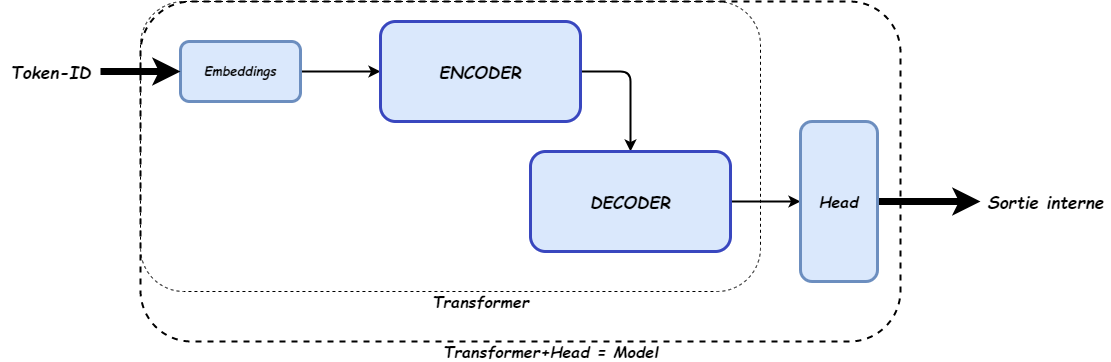
\includegraphics[width=16cm]{Model.png}
\captionof{figure}{Architecture interne du modèle mentionné sur la figure \ref{ArchiGloAbstract}}
\end{center}
$ _{ } $\\
Il s'agit en effet de l'architecture classique d'un \textit{transformer}, comme présenté sur la figure \ref{ImgTransformerVASWANI} à l'exception du fait qu'ici on fait ex\-pli\-ci\-te\-ment ap\-pa\-raî\-tre l'existence de la sortie du modèle. Ça correspond au \textit{réseau linéaire} suivi d'une couche de \textit{softmax} tel que présenté sur la figure \ref{ImgTransformerVASWANI}. Cette partie, que nous avons nommé \textit{head} est différente selon les tâches \cite{HF_wolf2020transformers}, c'est pourquoi nous avons voulu la mentionner explicitement car, selon le besoin, on peut la modifier.\\
Nous devons finalement mentionner que les modules de \textit{tokenisation} (nommés \textit{tokenizer} en anglais) dépendront explicitement des modèles utilisés.
\subsection{Présentation des interfaces}
$ _{} $ $ _{} $ $ _{} $ $ _{} $ $ _{} $La partie interface nous permettra juste d'utiliser le service que nous aurons élaboré et d'évaluer par la même occasion ses performances. Voici donc une ébauche d'interface que nous comptons utiliser pour exploiter le service :
$ _{ } $\\
\begin{center}
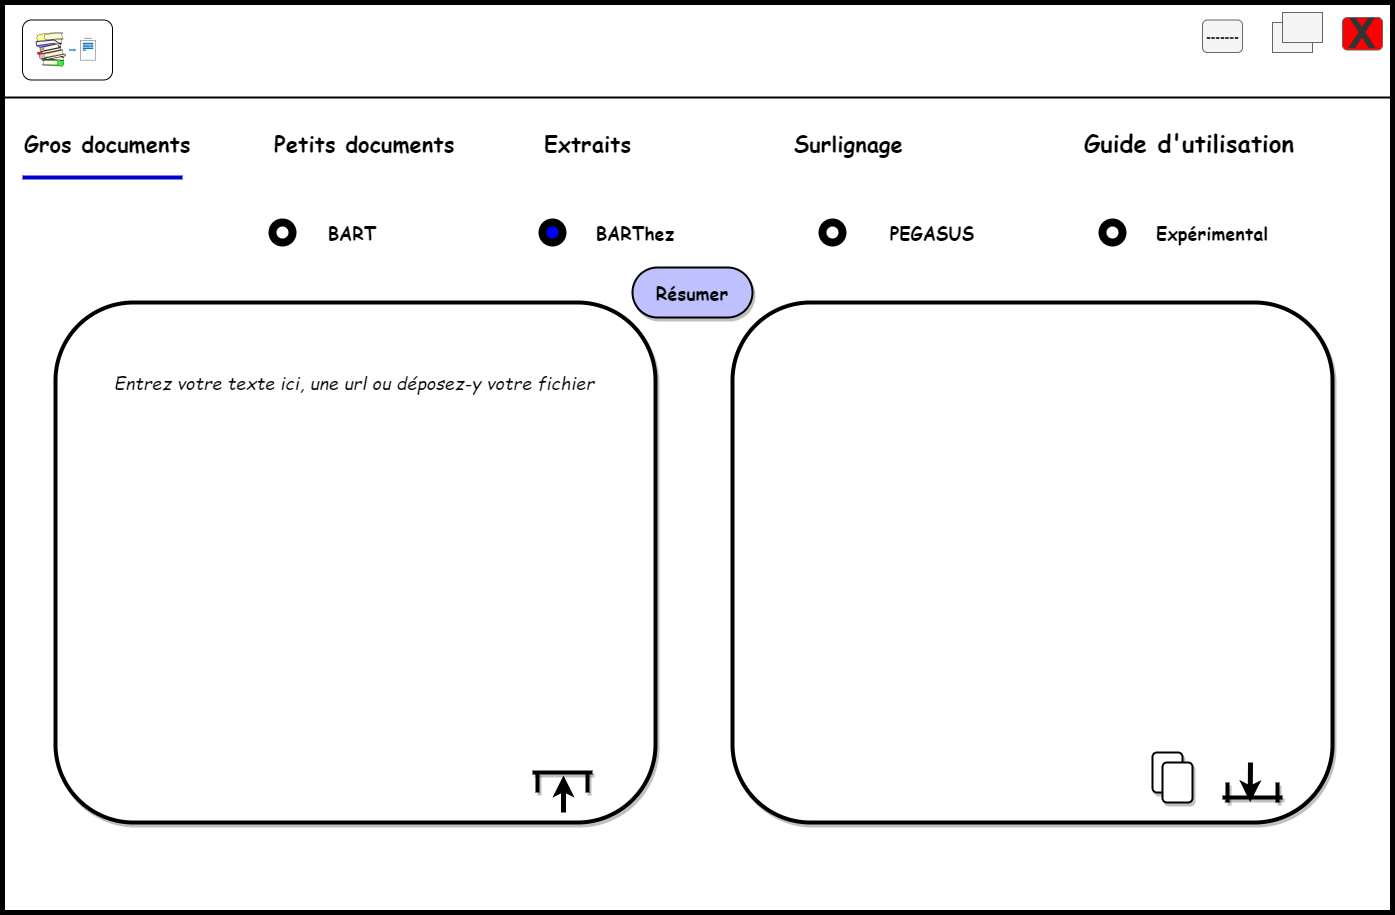
\includegraphics[width=16cm]{PageOne.png}
\captionof{figure}{Ébauche d'interface}\label{EbaucheInterface}
\end{center}
$ _{ } $\\
Avec cette interface, on a une idée générale de la manière dont nous comptons servir le système aux utilisateurs.
\section{Conclusion partielle}
$ _{} $ $ _{} $ $ _{} $ $ _{} $ $ _{} $Dans cette partie, nous venons de présenter le résumé automatique des textes, tout en réalisant une vue d'ensemble des méthodes utilisées dans la littérature à cet effet. Nous avons mentionné que la classification des résumés que nous utiliserons sera celle les départageant en \textit{abstractive summarization} et \textit{extractive summarization} et que, pour notre cas, il s'agira de réaliser un système de résumé mono-document, avec une partie abstractive et une autre extractive, générant un résumé générique pour des documents de type narratif et argumentatif.\\
$ _{} $ $ _{} $ $ _{} $ $ _{} $ $ _{} $Nous avons également listé les divers modèles de \textit{transformer} adaptés à la tâche de synthèse automatique abstraite, et nous avons mentionné devoir utiliser les modèles du type \textit{BART} pour des raisons qui serons précisées dans le chapitre suivant.\\
Enfin, nous avons réalisé la conception préliminaire du système tout en précisant que, concernant l'\textit{API}, la \textit{BD} (Base des Données) et les interfaces, les détails d'implémentation utiles seront précisés dans la partie dédiée à la conception proprement dite et aux tests, c'est-à-dire au chapitre suivant. Le chapitre suivant nous permettra donc finalement de préciser, réaliser et tester les méthodes que nous avons jusque-là adoptées pour la mise au point de notre système de synthèse automatique des documents.